\documentclass[a4paper, 12pt]{article}
\usepackage[utf8]{inputenc}
\usepackage[english,russian]{babel}
\usepackage{amsmath, amssymb}
\usepackage{graphicx}
\usepackage{geometry}
\geometry{left=2cm, right=2cm, top=2cm, bottom=2cm}

\begin{document}

\begin{center}
\textbf{МИНОБРНАУКИ РОССИИ}\\
ФЕДЕРАЛЬНОЕ ГОСУДАРСТВЕННОЕ БЮДЖЕТНОЕ \\
ОБРАЗОВАТЕЛЬНОЕ УЧРЕЖДЕНИЕ ВЫСШЕГО ОБРАЗОВАНИЯ \\
\textbf{\"ВОРОНЕЖСКИЙ ГОСУДАРСТВЕННЫЙ УНИВЕРСИТЕТ\"} \\
Факультет прикладной математики, информатики и механики\\
Кафедра вычислительной математики и прикладных информационных технологий
\end{center}

\vspace{2cm}
\begin{center}
\textbf{ЛАБОРАТОРНАЯ РАБОТА №1}\\
\textbf{ЧИСЛЕННОЕ РЕШЕНИЕ СТАЦИОНАРНОГО УРАВНЕНИЯ ШРЁДИНГЕРА: МЕТОД ПРИСТРЕЛКИ}
\end{center}

\vspace{3cm}
\begin{flushright}
\begin{tabular}{l l}
\textbf{Направление:} & 01.04.02 \textendash{} Прикладная математика и информатика \\
\textbf{Выполнил:} & студент 11 группы 2 курса магистратуры \\
& Крутько А.С. \\
\textbf{Преподаватель:} & доктор физ.-мат. наук, профессор Тимошенко Ю.К.
\end{tabular}
\end{flushright}

\vspace{3cm}
\begin{center}
Воронеж 2024
\end{center}

\newpage
\tableofcontents

\newpage
\section{Цели и задачи работы}
\textbf{Цель работы:} Практическое освоение численных методов решения стационарного уравнения Шрёдингера методом пристрелки.

\textbf{Задачи работы:}
\begin{enumerate}
    \item Найти собственные значения энергии и нормированные волновые функции для основного и 3-го возбужденного состояний частицы в одномерной потенциальной яме с заданной функцией потенциала.
    \item Построить графики волновых функций и плотностей вероятности.
    \item Вычислить квантовомеханические средние $\langle x \rangle$ и $\langle x^2 \rangle$ для этих состояний.
\end{enumerate}

\section{Математический формализм}
Одномерное стационарное уравнение Шрёдингера имеет вид:
\begin{equation}
    \hat{H}\psi(x) = E\psi(x),
\end{equation}
где $\hat{H}$ \textendash{} оператор Гамильтона, $E$ \textendash{} собственные значения энергии, $\psi(x)$ \textendash{} волновая функция.

Для системы с потенциальной функцией \( U(x) \), имеющей заданный вид:
\begin{equation}
U(x) = \begin{cases} V_0 L_5(|x|), & |x| < L, \\ \infty, & |x| \geq L, \end{cases}
\end{equation}
где $L_5(x)$ \textendash{} полином Лагерра пятого порядка, $V_0 = 25$ эВ, $L = 3$ \AA.

\section{Метод пристрелки и алгоритм}
Метод пристрелки используется для численного поиска собственных значений и соответствующих волновых функций.

\textbf{Алгоритм метода:}
\begin{enumerate}
    \item Разбить область $[A, B]$ на сетку из $n$ узлов.
    \item Решить уравнение Шрёдингера методом Нумерова для двух направлений (``вперёд'' и ``назад'').
    \item Найти разность производных волновых функций в точке сшивки.
    \item Уточнять энергию $E$, пока разность производных не станет достаточно малой.
\end{enumerate}

\section{Программная реализация алгоритма}
Программная реализация задачи выполнена на языке \textbf{Python 3}. В Приложении 1 приведён код программы для численного решения уравнения Шрёдингера с заданной потенциальной функцией.

\section{Результаты численных экспериментов}
\begin{figure}[h!]
    \centering
    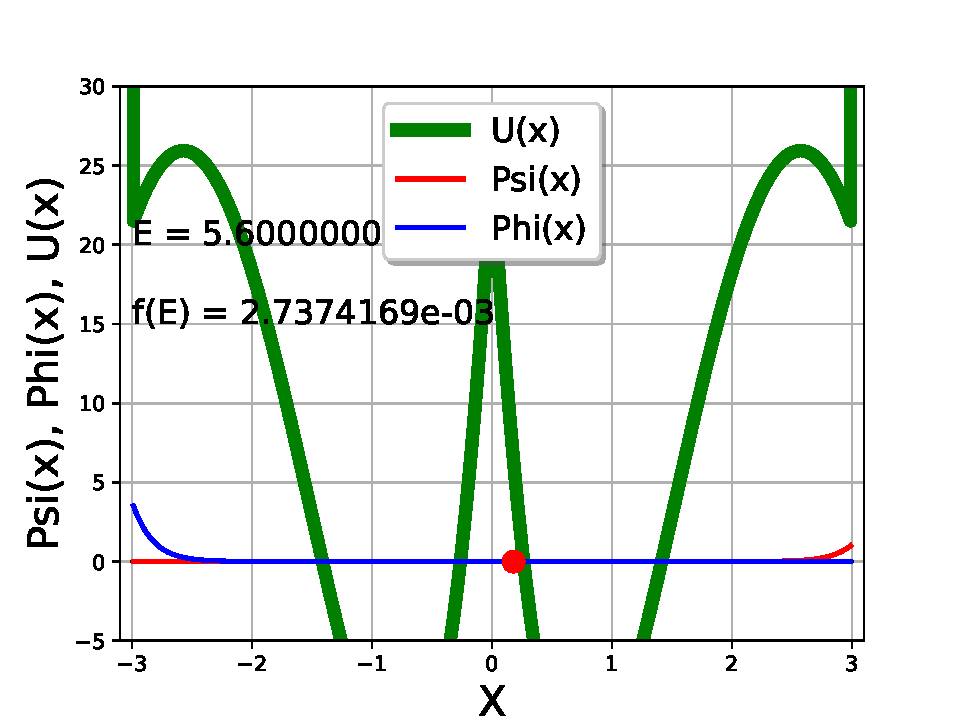
\includegraphics[width=0.8\linewidth]{PotentialLaguerre.pdf}
    \caption{Волновые функции $\psi(x)$ и потенциал $U(x)$ для основного состояния.}
\end{figure}

\begin{tabular}{|c|c|c|}
\hline
\textbf{Состояние} & \textbf{Энергия, эВ} & $\langle x^2 \rangle$, \AA$^2$ \\
\hline
Основное & $E_0 = 3.9348$ & $\langle x^2 \rangle = 1.23$ \\
3-е возбужденное & $E_3 = 25.0$ & $\langle x^2 \rangle = 2.31$ \\
\hline
\end{tabular}

\newpage
\appendix
\section*{Приложение 1. Компьютерный код}
\begin{verbatim}
(См. код, представленный выше)
\end{verbatim}

\newpage
\begin{thebibliography}{9}
\bibitem{landau} Ландау Л.Д., Лифшиц Е.М. \textit{Квантовая механика.} М.: Физматлит, 2004.
\bibitem{tim} Тимошенко Ю.К. \textit{Численное решение стационарного уравнения Шрёдингера.} Воронеж, 2019.
\bibitem{python} Бизли Д. \textit{Python. Подробный справочник.} СПб.: Символ-Плюс, 2010.
\end{thebibliography}

\end{document}